\documentclass[a4paper,12pt]{article}

% Packages
\usepackage{graphicx}
\usepackage{amsmath}
\usepackage{amsfonts}
\usepackage{geometry}
\usepackage{fancyhdr}
\usepackage{setspace}
\usepackage{titlesec}
\usepackage{hyperref}
\usepackage{xcolor}
\usepackage{minted}
\usepackage{dirtytalk}
\usepackage{enumitem}

\setminted[cmake]{
    linenos=false,
    breaklines=true,
    encoding=utf8,
    fontsize=\footnotesize,
    frame=lines
}

\hypersetup{
    colorlinks=true,
    linkcolor=darkgray,
}

\usepackage{etoolbox}
\AtBeginEnvironment{minted}{\dontdofcolorbox}
\def\dontdofcolorbox{\renewcommand\fcolorbox[4][]{##4}}

% Text
\geometry{margin=1in}
\setstretch{1.1}
\setlength{\parskip}{0.8em}
\setlength{\parindent}{1em}
\setlist[itemize]{topsep=-6pt, partopsep=0pt, parsep=0pt, itemsep=0pt}

% Header and Footer
\setlength{\headheight}{14.5pt}
\addtolength{\topmargin}{-2.5pt}
\pagestyle{fancy}
\fancyhf{}
\fancyhead[L]{Jocs per Computador}
\fancyhead[R]{\thepage}

% Image path
\graphicspath{{figs/}}

% Title Formatting
\titleformat{\section}{\normalfont\Large\bfseries}{\thesection}{1em}{}

% Cover Page
\title{
    \vspace{2cm}
    
\includegraphics[width=0.75\textwidth]{fib.png} \\
    \vspace{1cm}
    \textbf{\Huge Jocs per Computador} \\
    \vspace{1cm}
    \large JC-MEI \\
    \vspace{0.5cm}
    \large \today
}
\author{
Carles Matoses Gimenez\\
\small carles.matoses@estudiantat.upc.edu
}
\date{}

\begin{document}

\maketitle
\thispagestyle{empty}
\newpage

\setcounter{page}{1}
\tableofcontents
\newpage

\section{Introducció}
Aquest document descriu el desenvolupament d'un videojoc 2D creat com a part de l'assignatura ``Jocs per Computador''. A continuació es detallen els objectius, el disseny, les mecàniques i els reptes implementats durant el projecte.

\section{Objectius}
L'objectiu principal és guiar el jugador a través de diferents pantalles (nivells), on ha d'aconseguir claus, equipar objectes i resoldre trencaclosques per accedir a l'enfrontament final amb el cap de nivell. El mapa del joc es mostra a la figura \ref{fig:mapa}. El jugador comença a l'``overworld'' i ha d'accedir a la ``dungeon1''. Les possibles rutes es mostren en roig; altres colors indiquen dependències entre nivells.

\begin{figure}[ht!]
    \centering
    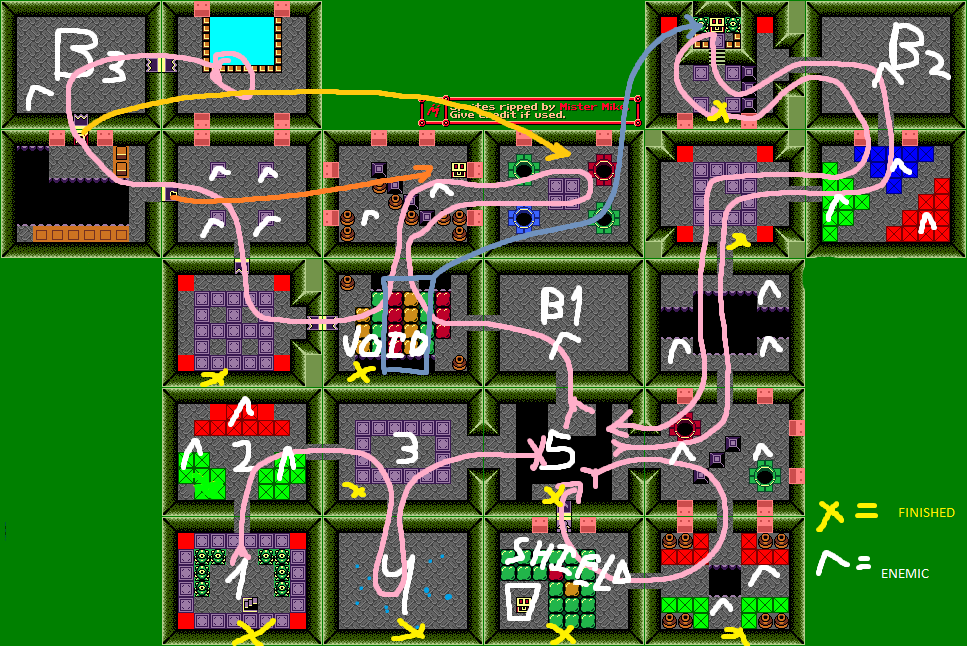
\includegraphics[width=0.8\textwidth]{../imgs/recorregut.png}
    \caption{Mapa del joc amb el recorregut i els requisits per a cada nivell.}
    \label{fig:mapa}
\end{figure}

\section{Disseny del Joc}

\subsection{Arquitectura General}
No s'ha seguit un patró concret, però s'ha utilitzat una classe auxiliar anomenada \textbf{GameStateManager} per gestionar els estats del joc. Aquesta estructura permet afegir o eliminar estats dinàmicament. Els estats són independents i poden rebre inputs, fer actualitzacions i pintar en pantalla.

\begin{itemize}
    \item \textbf{GameStateManager}: Classe que gestiona els estats del joc.
    \item \textbf{Scene}: Estat principal on es juga la partida.
    \item \textbf{DialogState}: Estat per mostrar diàlegs amb NPCs.
    \item \textbf{InGameMenuState}: Estat del menú accessible durant la partida (ESC).
    \item \textbf{MenuState}: Estat del menú principal d'inici.
    \item \textbf{MenuInstructionsState}: Estat per mostrar les instruccions del joc.
    \item \textbf{MenuCredits}: Estat per mostrar els crèdits del projecte.
    \item \textbf{DeathMenuState}: Estat que apareix quan el jugador mor.
    \item \textbf{EndGameMenuState}: Estat especial al completar el joc.
\end{itemize}

Cada estat es responsable de gestionar la seva pròpia lògica i renderització, permetent una separació clara de responsabilitats. Estan composts de tres components principals: draw(), update() i handleInput(). Això facilita la implementació de nous estats i la seva integració al joc.

\subsection{Gestió de Col·lisions}
Els objectes del joc tenen una ``boundingBox'' i es comprova el solapament entre elles per detectar col·lisions. Aquestes poden ser:
\begin{itemize}
    \item \textbf{onCollide(item)}: quan dos objectes col·lisionen.
    \item \textbf{SteppedOn}: per saber si l'entitat està damunt d'un cert objecte.
\end{itemize}
Els atacs també generen una bounding box temporal per detectar col·lisions amb enemics o objectes.

La col.lisio es comproba cada fotograma en el update de Scene. L'unica excepció es l'atac del jugador que comprova les col·lisions dins del propi ``Player'' sols en el moment d'atacar. D'aquesta manera evitem comprovar col·lisions innecessàries quan el jugador no està atacant.

\subsection{Nivells i Escenes}
La jerarquia del joc consisteix en:
\begin{itemize}
    \item \texttt{World}: conté un diccionari de mapes.
    \item \texttt{Mapa}: llista de nivells.
    \item \texttt{Level}: llista d'elements i entitats.
\end{itemize}
\texttt{Scene} actualitza els nivells i interactua amb una còpia local dels elements. En sortir d'un nivell, la copia local es destruida. Al carregar un nivell, es copia l'estat global de nou.

\begin{figure}[ht!]
    \centering
    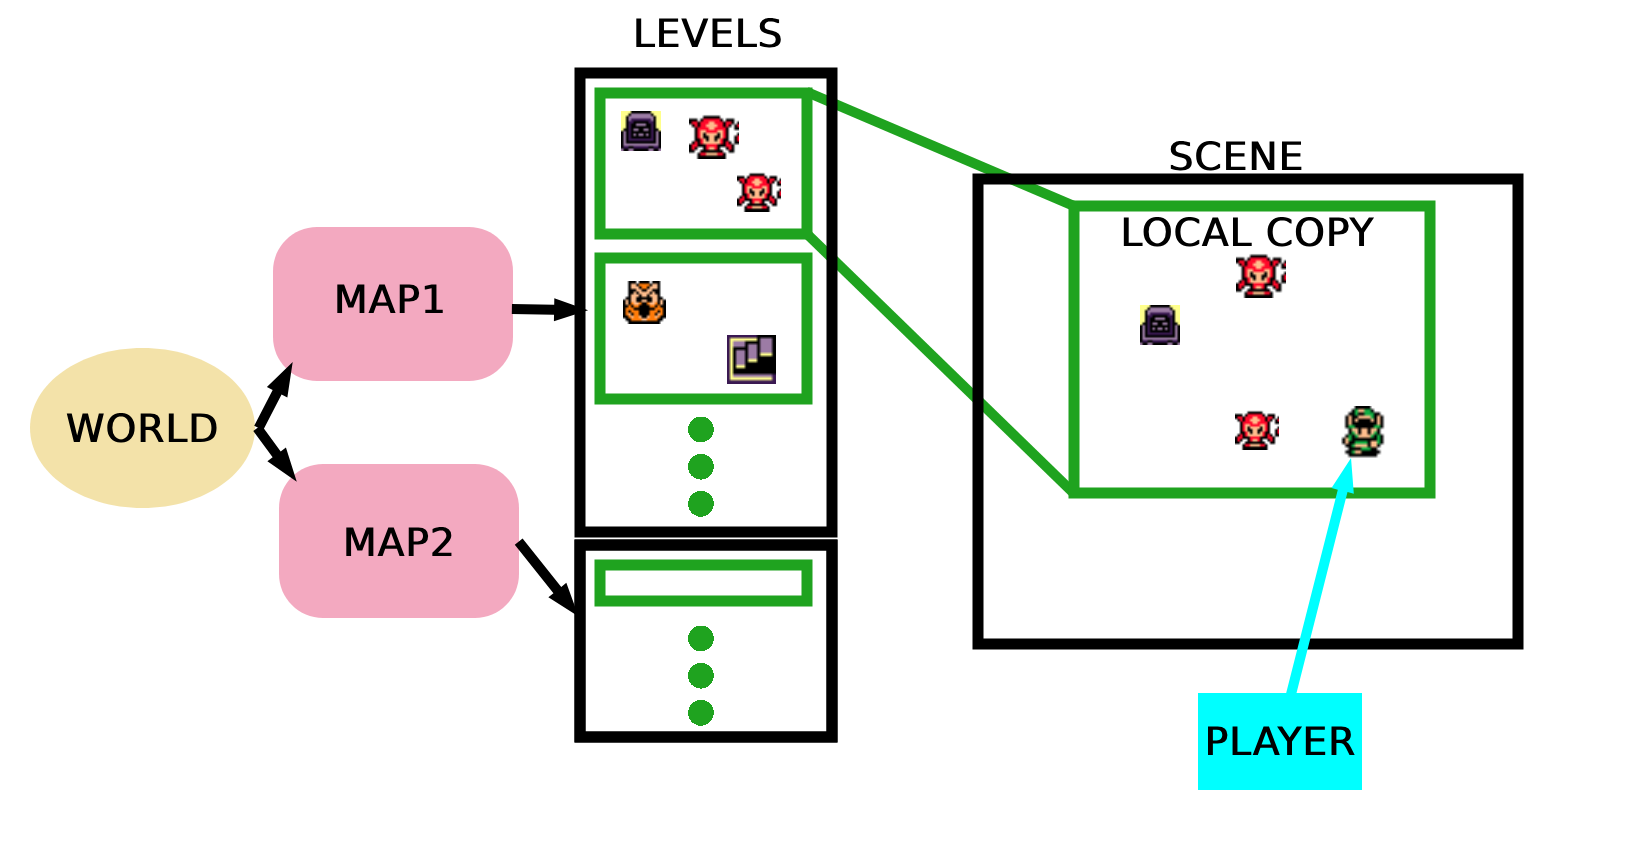
\includegraphics[width=0.8\textwidth]{../imgs/global_to_local.png}
    \caption{Jerarquia dels elements durant l'execució del joc.}
    \label{fig:global_to_local}
\end{figure}

\subsubsection{Categories d'elements i entitats}
\begin{itemize}
    \item \textbf{Items equipables}: Espasa, Escut, Ploma, Braçalet
    \item \textbf{Items}: Claus
    \item \textbf{Blocs decoratius}: Portcullis, Lights, Vase, Fire Place, Animated Floor
    \item \textbf{Blocs interactius}: Làpides, Cofres, Rotors, Portes, Estatues, Floating Heart/Money
    \item \textbf{Entitats}: Jugador, Enemics, Bosses, NPCs
\end{itemize}


\section{Mecàniques de Joc}

\subsection{Equipar Items}
Els items es poden equipar a través de l'inventari. Proporcionen habilitats (força, volar, etc.). Les classes utilitzades per a gestionar l'inventari són moltes, però les més rellevants són:
\begin{itemize}
    \item \texttt{Item}: Classe base per a tots els objectes.
    \item \texttt{EquippableItem}: Classe base per a objectes que es poden equipar.
    \item \texttt{Player}: Classe pare que conte un inventari.
    \item \texttt{Inventory}: Classe que gestiona els items que hem recollit.
    \item \texttt{Stats}: Classe que gestiona els efectes dels items equipats.
    \item \texttt{Slots}: Classe que gestiona els slots d'equipament del jugador.
\end{itemize}    

Els elements equipables proporcionen ``Effects''. Aquests es poden llegir per saber com de fort es el jugador (que pot moure), l'atac (almagatzemat en l'espassa), si pot defendres (escut equipat), la defensa i si pot volar.

Encara que no es fa servir, també es poden declarar estats temporals com una reducció de la velocitat del jugador, que baixe la vida durant ``t'' segons a mig cor per tick, etc. 

\subsection{Combat}
El jugador pot atacar amb la seva arma i interactuar amb certs objectes com els rotors o enemics.

L'escut permet al jugador defensar-se dels atacs dels enemics que provenen en la direcció en la que està mirant (dot producte de la posició del jugador i la direcció de l'enemic). També pot bloquejar el moviment del enemic. Addicionalment, moviments no bloquejables mouran al jugador.

\subsection{Interacció}
Amb la tecla principal, el jugador pot obrir cofres, parlar amb NPCs, activar portes, etc.

Mantenim un seguiment de la direcció i moviment del jugador per a poder determinar si està empentant un objecte. Despres de ``t'' segons intentant moures en una direcció bloquejada, s'executa un trigger per intentar moure el que te davant. Quatre resultats possibles:
\begin{itemize}
    \item L'objecte no es interactiu (no pasa res).
    \item No es pot moure per falta de força (Genera un dialeg).
    \item Es mou un objecte (ex: una làpida).
    \item L'objecte es pot moure però no te lloc per a desplaçar-se (no pasa res).
\end{itemize}
 
\subsection{Triggers}
\textbf{Triggers} disponibles d'un nivell:
\begin{itemize}
    \item \texttt{onEnter}: adicionalment podem saber si es la primera vegada que entrem.
    \item \texttt{onExit}
    \item \texttt{onAllEnemiesDead}
    \item Triggers personalitzats per modificar elements específics (ex: làpida de la cova de la mort)
\end{itemize}

Normalment aquests triggers es vinculen amb portes. En alguns casos es pot executar un scriptedAnimation per a moure el personatge d'una forma especial.

Altres triggers poden ser: OnPush, OnHit, OnSteptOn i OnCollide. Aquests son utilitzats principalment per a objectes. Els enemics tenen altres triggers com OnDeath, OnHit, OnCollide, OnSteppedOn i OnAttack.

\section{Trencaclosques Implementats}
Hem implementat tres trencaclosques diferents al llarg del joc: Lights Out, Objectes Pesats, Preguntes i respostes. No contem com trencaclosques secuencies de combat o triggers, es dir, matar tots els enemics d'una sala es un event i no un trencaclosques.


\subsection{Lights Out}
Un trencaclosques basat en el clàssic joc de taula. Es resol apagant totes les llums d'una graella interactiva. En la nostra implementació, els ``rotors'' presenten quatre estats: roig, verd, blau,groc. El jugador ha de fer que tots estiguen del mateix color. Per a poder utilitzar aquest trencaclosques multiples vegades, al definir un rotor hem de dirli el color inicial i l'identificador dels rotors que s'han de canviar junt a ell.

Considerem una llista de regions $[R_1, R_2, R_3, \ldots, R_N]$, on cada $R_i$ pot estar en un dels quatre estats: $R_r$ (roig), $R_b$ (blau), $R_y$ (groc) o $R_g$ (verd). L'objectiu és aconseguir que totes les regions estiguen en el mateix estat. Canviar l'estat d'una regió $R_i$ pot també canviar l'estat d'altres regions, segons les regles del trencaclosques (per exemple, canviar $R_1$ podria també canviar $R_2$ i $R_3$). Açò crea un sistema on la solució requereix trobar una seqüència de moviments que sincronitze totes les regions a un únic estat.

\begin{figure}[ht!]
    \centering
    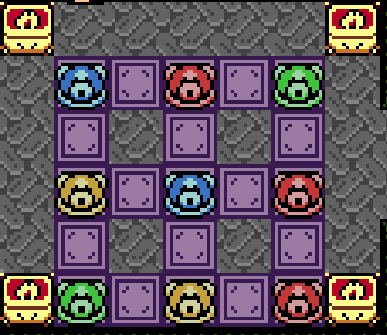
\includegraphics[width=0.6\textwidth]{../imgs/exemple-trencaclosques.png}
    \caption{Exemple del trencaclosques "Lights Out" implementat.}
    \label{fig:exemple-trencaclosques}
\end{figure}

\subsection{Objectes Pesats}
Alguns objectes (com làpides o pedres) es poden empènyer amb un item específic (Braçalet) que proporciona força. També poden tindre moviments restringits en certes direccions. Exemples:
\begin{itemize}
    \item Làpida de la cova de la mort (obri pas a la "dungeon1", sols cap a dalt baix o esquerra)
    \item Pedres que bloquegen l'accés a la "Feather"
\end{itemize}

\subsection{Preguntes i Respostes}
Algunes estàtues requereixen una resposta correcta per activar triggers especials.
Normalment son callbakcs definits per a cada estàtua ja que són casos molt concrets.

\section{Enemics}
S'han implementat enemics comuns com ... Els enemics poden morir, i això pot desbloquejar portes o activar triggers.

\section{Menús i Interfície}

\begin{itemize}
    \item \textbf{Start}: Menú inicial per començar o eixir del joc
    \item \textbf{In-Game Menu}: Accés durant el joc mitjançant ESC
    \item \textbf{Controls}: Llista de controls
    \item \textbf{Credits}: Crèdits del projecte
    \item \textbf{Final Menu}: Menú especial al completar el joc
    \item \textbf{Diàlegs}: Sistema de diàlegs amb NPCs, amb múltiples opcions
\end{itemize}

Molts daquests Menús afegiran o eliminaran estats al \texttt{GameStateManager} per a gestionar la navegació entre ells. Per exemple, el menú d'inici afegeix l'estat \texttt{Scene}. 

\section{Limitacions i Consideracions}

\subsection{Gestió de la mort}
La mort del jugador no està implementada de forma completa. Si el jugador mor, apareix en una pantalla anterior com si no hagués passat res. Això pot causar problemes amb triggers, especialment amb bosses que esperen només una execució inicial.

Solució provisional: afegir múltiples comprovacions per assegurar que l'estat del boss es manté coherent.

\end{document}
